\documentclass{article}

% Language setting
% Replace `english' with e.g. `spanish' to change the document language
\usepackage[english]{babel}

% Set page size and margins
% Replace `letterpaper' with `a4paper' for UK/EU standard size
\usepackage[letterpaper,top=2cm,bottom=2cm,left=3cm,right=3cm,marginparwidth=1.75cm]{geometry}

% Useful packages
\usepackage{amsmath}
\usepackage{amssymb}
\usepackage{graphicx}
\usepackage[colorlinks=true, allcolors=blue]{hyperref}

\begin{document}

\section{CERN, the LHC, and the CMS Experiment}

\subsection{CERN and the Large Hadron Collider}
% [CITE] https://cds.cern.ch/record/782076
The European Council for Nuclear Research (in French \textit{Conseil Europ\'{e}en pour la Recherche Nucl\'{e}aire}), also known as CERN, is the site of an accelerator complex hosting the Large Hadron Collider (LHC). The LHC consists of a 27-kilometer ring of superconducting magnets with accelerating structures to boost the energy of particles, which collide at a center-of-mass energy of up to 14 TeV. The beams inside the LHC are made to collide at four locations around the accelerator ring, at the locations of four particle detectors: ATLAS, CMS, ALICE, and LHCb.

The number of events generated per second at the LHC collisions is given by $N_{event} = \mathcal{L} \sigma_{event}$, where $\sigma_{event}$ is the cross-section for the event under study, and $\mathcal{L}$ the machine luminosity. The machine luminosity depends only on the beam parameters, and can be written for a Gaussian beam distribution as:

\begin{equation}
    \mathcal{L} = \frac{N_b^2 n_b f_{rev} \gamma_r}{4\pi \epsilon_n \beta^*} F
\end{equation}
where $N_b$ is the number of particles per bunch, $n_b$ the number of bunches per beam, $f_{rev}$ the revolution frequency, $\gamma_r$ the relativistic gamma factor, $\epsilon_n$ the normalized transverse beam emittance, $\beta^*$ the beta function at the collision point, and $F$ the geometric luminosity reduction factor due to the crossing angle at the interaction points. Luminosity is measured in units of cm$^{-2}$ s$^{-1}$. Thus the exploration of rare events in the LHC collisions requires both high beam energies and high beam intensities.

\subsection{The CMS Detector}
\label{section:cms-detector}

\begin{figure}[ht]
    \centering
    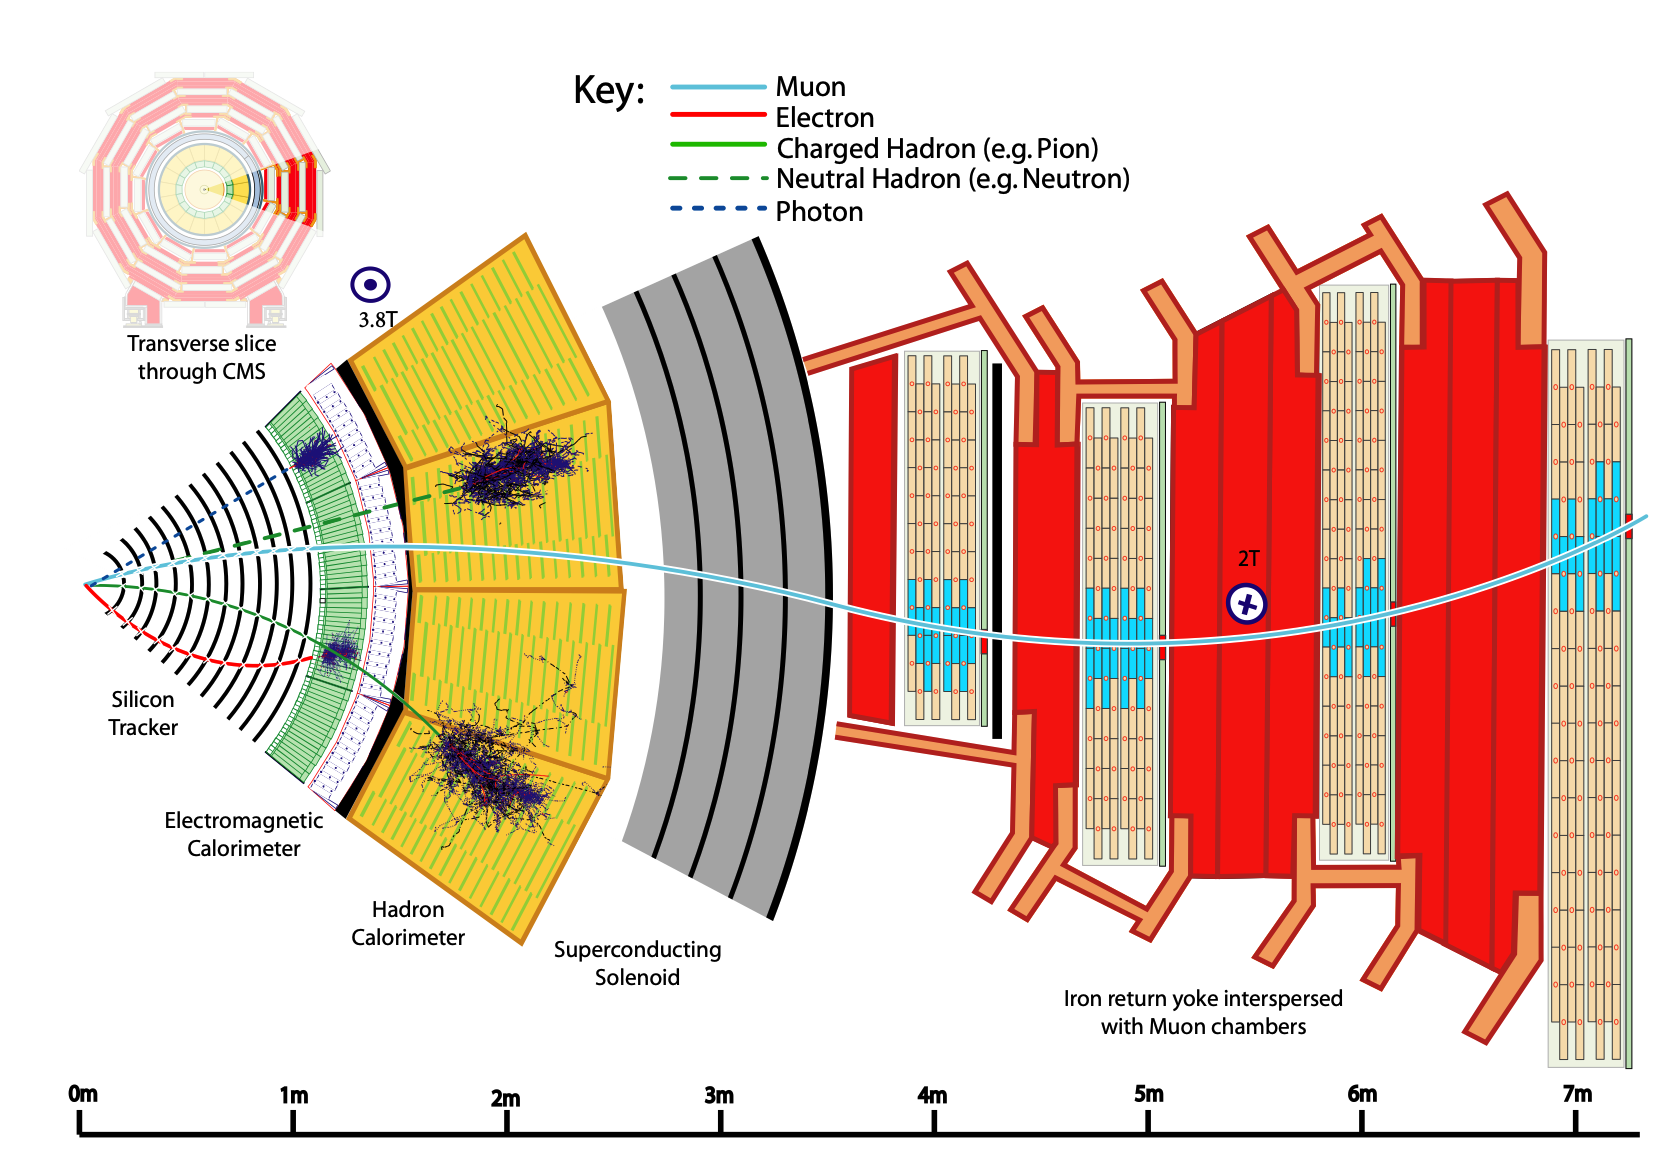
\includegraphics[width=11cm]{figures/sketch-cms-particle-interactions.png}
    \caption{Sketch of particle trajectories of muons, electrons, charged and neutral hadrons, and photons in a transverse cross-section of the CMS detector, from [CITE] https://arxiv.org/pdf/1706.04965.pdf.}
    \label{fig:sketch-cms-particle-interactions}
\end{figure}

% cite https://iopscience.iop.org/article/10.1088/1748-0221/3/08/S08004/pdf
% cite https://arxiv.org/pdf/1706.04965.pdf 
The Compact Muon Solenoid (CMS) experiment was conceived to study proton-proton and lead-lead collisions at a center-of-mass energy of 14 TeV (5.5 TeV nucleon-nucleon) and at luminosities up to $10^{34}$ cm$^{-2}$ s$^{-1}$ ($10^{27}$ cm$^{-2}$ s$^{-1}$). Starting from the beam interaction region at the center of the CMS detector, particles first pass through a silicon pixel and strip tracker, in which charged-particle trajectories (tracks) and origins (vertices) are reconstructed from signals (hits) in the sensitive layers. The tracker is immersed in a high-magnetic-field superconducting solenoid that bends the trajectories of charged particles, allowing the measurement of their electric charge and momenta. Electrons and photons are then absorbed in an electromagnetic calorimeter (ECAL) comprised of lead-tungstate scintillating-crystals. The corresponding electromagnetic showers are detected as clusters of energy recording in neighboring cells, from which the direction and energy of the particles can be determined. Charged and neutral hadrons may initiate a hadronic shower in the ECAL as well, which is then fully absorbed in the hadron calorimeter (HCAL). The resulting clusters are used to estimate their direction and energies. Muons and neutrinos pass through the calorimeters with little to no interactions. Neutrinos escaped undetected; muons produce hits in additional gas-ionization chamber muon detectors housed in the iron yoke of the flux-return. A sketch of example particle interactions in a transverse slice of the CMS detector is shown in Fig. \ref{fig:sketch-cms-particle-interactions}. The collision data is recorded with the use of the Level-1 (L1) trigger, high-level trigger (HLT), and data acquisition systems ensuring high efficiency in selecting physics events of interest. 


% not super clean citation: Tracker TDR https://cds.cern.ch/record/2272264/files/CMS-TDR-014.pdf
CMS uses a right-handed coordinate system [CITE]. The origin is centered at the nominal collision point inside the experiment. The $x$ axis points towards the center of the LHC, and the $y$ axis points vertically upwards. The $z$ axis points along the beam direction. The azimuthal angle, $\phi$, is measured from the $x$ axis in the $x$-$y$ plane, and the radial coordinate in this plane is denoted by $r$. The polar angle, $\theta$, is measured from the $z$ axis. The pseudorapidity, $\eta$, is defined as $\eta = -\ln \tan(\theta/2)$. The momentum and energy transverse to the beam direction, denoted by $p_{T}$ and $E_{T}$ respectively, are computed from the $x$ and $y$ components. The momentum imbalance in the transverse plane is called the missing transverse momentum, and its magnitude is denoted by $E_{T}^{\text{miss}}$.

\subsection{Sub-detectors of CMS}
This section details the sub-detectors of CMS that operate to identify and precisely measure muons, electrons, photons, and jets over a large energy range. 

\subsubsection{Inner tracking system}
% CITE: Original Tracker TDR https://cds.cern.ch/record/368412/files/Tracker_TDR.pdf
% CITE: Phase-1 Tracker TDR: https://cds.cern.ch/record/1481838 
% CITE: Phase-2 https://cds.cern.ch/record/2272264/files/CMS-TDR-014.pdf
The CMS Tracker perform robust tracking and detailed vertex reconstruction in the 4 T magnetic field of the superconducting solenoidal magnet. The active envelope of the CMS Tracker extends to a radius of 115 cm, over a length of approximately 270 cm on each side of the interaction point [CITE] %original tracker TDR. 
Charged particles in the region $|\eta| \lesssim 1.6$ benefit from the full momentum measurement precision. In this region, a charged particle with $p_T$ of 1000 GeV has a sagitta of $\sim 195$ $\mu$m. The Tracker acceptance extends further to $|\eta| = 2.5$, with a reduced radial lever arm of approximately 50 cm.

The high magnetic field of CMS causes low $p_{T}$ charged particles to travel in helical trajectories with small radii. The majority of events contain particles with a steeply falling $p_{T}$ spectrum, resulting in a track density which rapidly decreases at higher radii. 

\begin{figure}[ht]
    \centering
    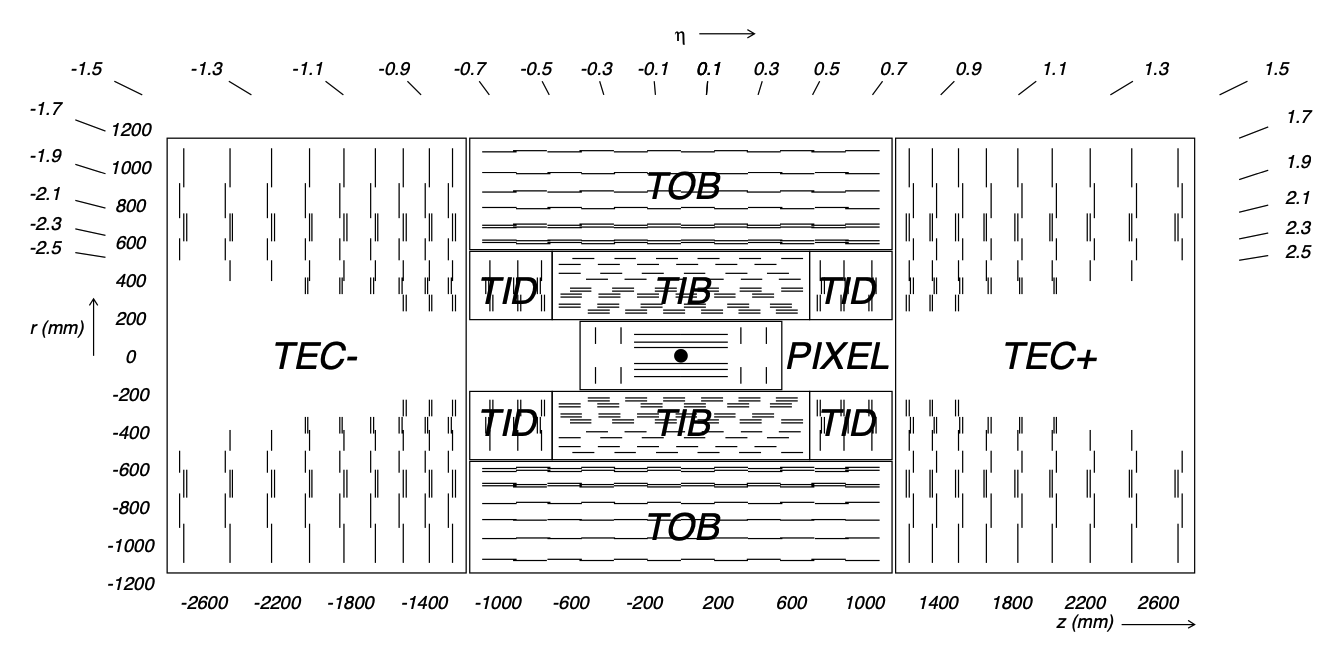
\includegraphics[width=11cm]{figures/phase-1-tdr-tracker-schematic.png}
    \caption{Cross section of the current Phase-1 CMS tracker from [CITE] https://cds.cern.ch/record/1481838/files/CMS-TDR-011.pdf, showing the nomenclature of different sections. Each line represents a detector module. Double lines indicate back-to-back modules which deliver stereo hits in the strip tracker.}
    \label{fig:phase-1-tdr-tracker-schematic}
\end{figure}


A schematic view of the current Phase-1 CMS tracker, including the pixel detector, is shown in Fig. \ref{fig:phase-1-tdr-tracker-schematic}. The Phase-1 pixel detector consists of three barrel layers (BPIX) at radii of 4.4 cm, 7.3 cm, and 10.2 cm, and two forward/backward disks (FPIX) at longitudinal positions of $\pm$ 34.5 cm and $\pm$ 46.5 cm, and extending in radius from about 6 cm to 15 cm. These pixelated detectors produce 3D measurements along the paths of charged particles with single hit resolutions between 10-20 $\mu$m. 

% here cite 2008 JINST 3 S08004 https://iopscience.iop.org/article/10.1088/1748-0221/3/08/S08004/pdf
After the pixel and on their way out of the tracker, particles pass through the silicon strip tracker which reaches out to a radius of 130 cm (Fig. \ref{fig:phase-1-tdr-tracker-schematic}). The sensor elements in the strip tracker are single-sided $p$-on-$n$ type silicon micro-strip sensors [CITE 2008 CMS]. The silicon strip detector consists of four inner barrel (TIB) layers assembled in shells, with two inner endcaps (TID), each composed of three small discs. The outer barrel (TOB) consists of six concentric layers. Two endcaps (TEC) close off the tracker on either end. 


\subsubsection{ECAL} 
% cite again 2008 JINST 3 S08004: https://iopscience.iop.org/article/10.1088/1748-0221/3/08/S08004/pdf
The electromagnetic calorimeter (ECAL) of CMS measures electromagnetic energy deposits with high granularity. One of the driving criteria in the design was the capability of detecting the Standard Model Higgs boson decay to two photons (in fact, the channel in which the 125 GeV Higgs boson was discovered at CMS).

% cite PDG Passage of Particles THrough Materal: https://pdg.lbl.gov/2019/reviews/rpp2018-rev-passage-particles-matter.pdf
High-energy electrons predominantly lose energy in matter via bremsstrahlung, and high-energy photons by $e^+ e^-$ pair production. The characteristic amount of matter traversed for these interactions is called the radiation length $X^0$, usually measured in units of g cm$^-2$. It is the mean distance over which a high-energy electron loses all but $1/e$ of its energy via bremsstrahlung [CITE PDG]. 

% back to 2008 JINST 3 S08004
ECAL is a hermetic homogenous calorimeter comprised of 61,200 lead tungstate (PbWO$_4$) crystals mounted in the central barrel, with 7,324 crystals in each of the two endcaps [CITE]. A preshower detector is located in front of the endcap crystals. Avalanche photodiodes (APDs) are used as photodetectors in the barrel and vacuum phototriodes (VPTs) in the endcaps. 

% back to 2008 JINST 3 S08004
The barrel part of the ECAL (EB) covers the pseudorapidity range $|\eta| < 1.479$. The barrel granularity is 360-fold in $\phi$ and ($2 \times 85$)-fold in $\eta$. The crystal cross-section corresponds to approximately $0.0174 \times 0.0174$ in $\eta-\phi$ or $22 \times 22$ mm$^2$ at the front face of the crystal, and $26 \times 26$ mm$^2$ at the rear face. The crystal length is 230 mm, corresponding to 25.8 $X_0$.

% 2008 JINST 3 S08004
The ECAL read-out acquires the signals of the photodetectors. At each bunch crossing, digital sums representing the energy deposit in a trigger tower, comprising $5 \times 5$ crystals in $\eta \times \phi$, are generated and sent to the Level-1 trigger system (detailed in Section \ref{section:phase-1-l1-trigger}).

\subsubsection{HCAL}
\begin{figure}[ht]
    \centering
    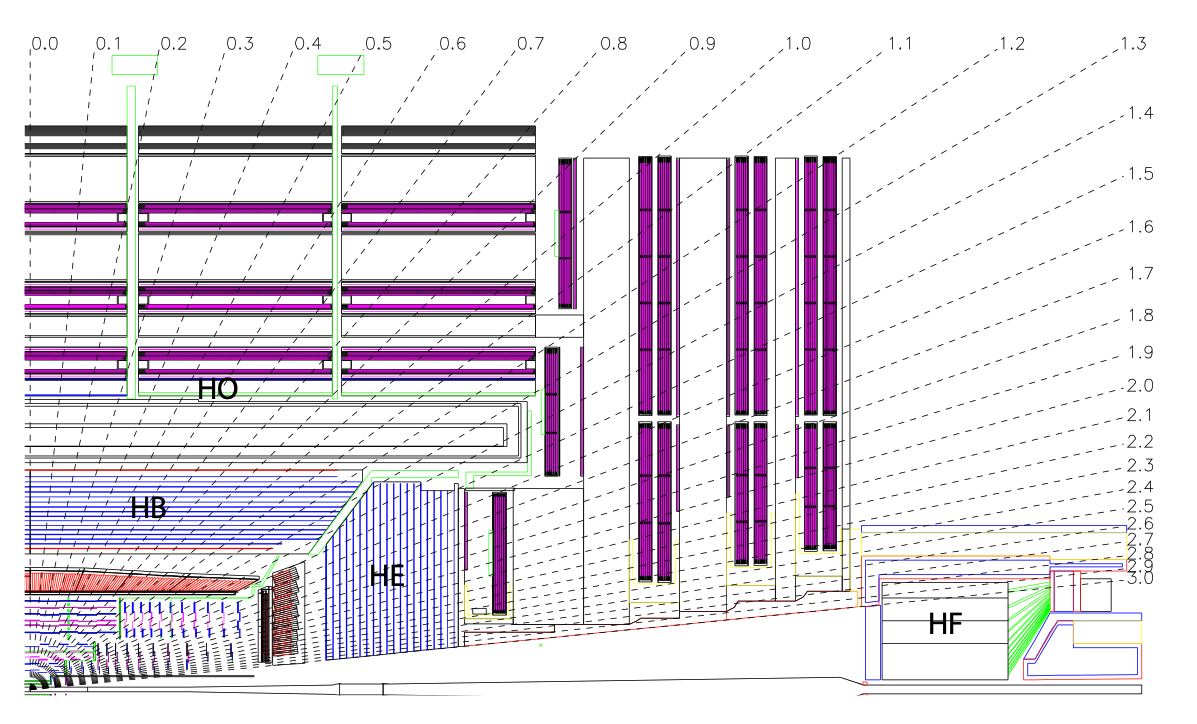
\includegraphics[width=11cm]{figures/phase-1-HCAL-schematic.png}
    \caption{Longitudinal view of the CMS detector showing the hadron calorimeter barrel (HB), endcap (HE), outer (HO), and forward (HF) calorimeters from [CITE 2008 JINST 3 S08004].}
    \label{fig:phase-1-HCAL-schematic}
\end{figure}

% 2008 JINST 3 S08004
The hadronic calorimeter (HCAL) of CMS plays an important role in the measurement of hadron jets and neutrinos or exotic particles resulting in apparent missing transverse energy. A view of the CMS detector showing the components of HCAL is shown in Fig. \ref{fig:phase-1-HCAL-schematic}. The HCAL barrel (HB) and endcaps (HE) are located outside of the tracker and the ECAL. The hadron calorimeter barrel is radially restricted between the outer radius of the electromagnetic calorimeter at a radius of 1.77 m, and the inner extent of the magnet coil at radius 2.95 m. An outer hadron calorimeter (HO) is placed outside the solenoid to complement the barrel calorimeter. Beyond $|\eta| = 3$, the forward hadron calorimeter (HF) at 11.2 m from the interaction point extend the pseudorapidity coverage to $|\eta| = 5.2$.

% 2008 JINST 3 S08004
The HB is a sampling calorimeter covering the pseudorapidity range $|\eta| < 1.3$. It consists of 36 identical azimuthal wedges which form two half-barrels (HB+ and HB-). Each wedge is segmented into four azimuthal angle ($\phi$) sectors. The plastic scintillator is divided into 16 $\eta$ sectors, resulting in a segmentation of $(\Delta \eta, \Delta \phi) = (0.087, 0.087)$. The HE covers pseudorapidity $1.3 < |\eta| < 3$, and the design is driven by the need to minimize the cracks between HB and HE, rather than single-particle energy resolution, since the resolution of jets in HE will be limited by pileup, magnetic field effects, and parton fragmentation. 

% 2008 JINST 3 S08004
In the central pseudorapidity region, the combined stopping power of EB plus the HB is insufficient to contain hadron showers [CITE]. To ensure adequate sampling depth, the hadron calorimeter is extended with a tail catcher, the HO. The size and position of the tiles are designed to roughly map the layers of the HB to make towers with the same granularity of $0.087 \times 0.087$ in $\eta$ and $\phi$. The HO is physically divided in 5 rings in $\eta$ conforming to the muon ring structure. 

% 2008 JINST 3 S08004
The HF is foremost designed to survive in the harsh radiation conditions and high particle flux of the forward region. On average, 760 GeV per proton-proton interaction is deposited into the two forward calorimeters, compared to only 100 GeV for the rest of the detector [CITE]. Furthermore, this energy has a pronounced maximum at the highest rapidities. As a result of these radiation considerations, quartz fibers are used as the active medium. The signal is generated when charged shower particles above the Cherenkov threshold 

\subsubsection{Muon detectors}

% 2008 JINST 3 S08004
The CMS muon system is designed to have the capability of reconstructing the momentum and charge of muons over the kinematic range of the LHC, since muons are a powerful handle on signatures of interesting processes over the high background rate of the LHC. For instance, the decay of the Standard Model Higgs boson into $ZZ$, which in turn decay to 4 leptons, can be reconstructed with high 4-particle mass resolution if all the leptons are muons, since muons are less affected than electrons by radiative losses in the tracker material. The muon system consists of a cylindrical barrel section and two planar endcap regions.

\begin{figure}[ht]
    \centering
    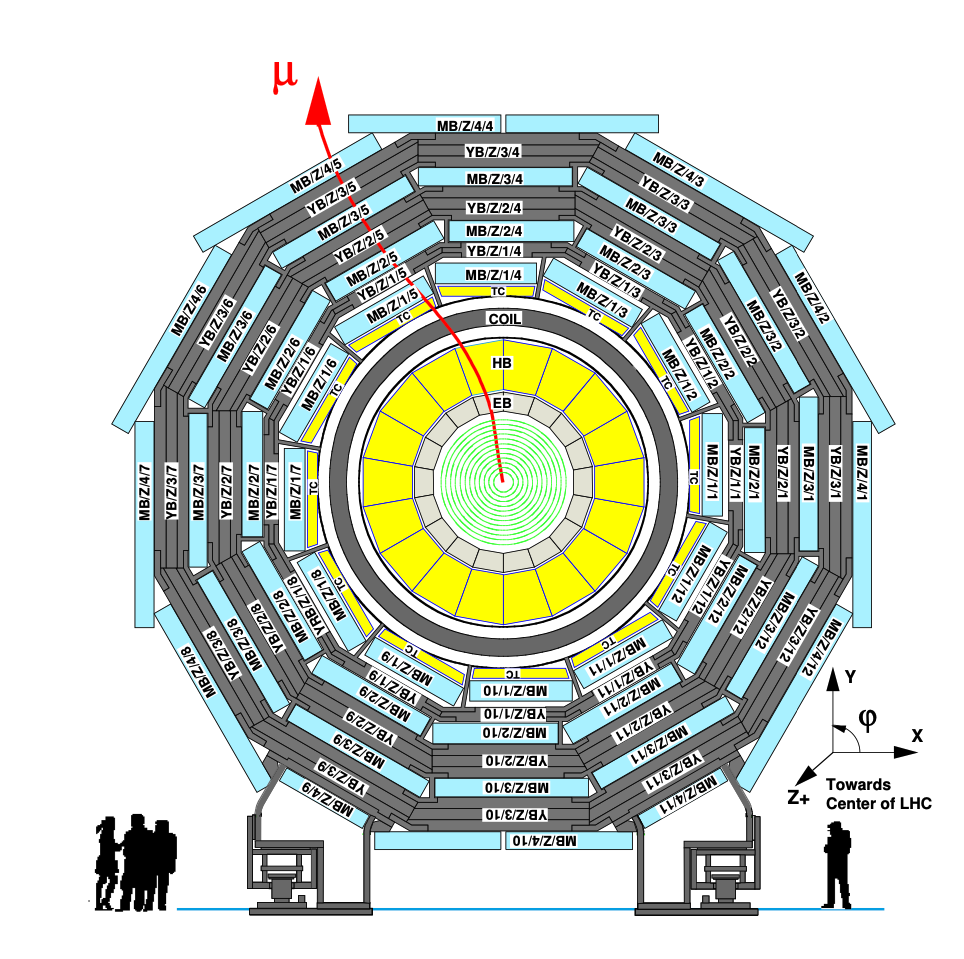
\includegraphics[width=11cm]{figures/phase-1-muon-barrel-DT-schematic.png}
    \caption{Layout of the CMS barrel muon DT chambers in one of the five wheels from [CITE 2008 JINST 3 S08004].}
    \label{fig:phase-1-muon-barrel-DT-schematic}
\end{figure}

% 2008 JINST 3 S08004, page 165
The barrel muon detector deploys drift tube (DT) chambers covering the pseudorapidity region $|\eta| < 1.2$. In the barrel region, the neutron-induced background is small, the muon rate is low, and the 4T magnetic field is uniform and mostly contained in the steel yoke. The low expected rate allows the use of the DTs as tracking detectors for the barrel muon system. A DT chamber is made of 3 or 2 superlayers, each made of 4 layers of rectangular drift cells staggered by a cell. Since two detector layers (one inside the yoke and the other outside) would be insufficient for reliable identification and identification, two additional layers of DTs are embedded within the yoke iron. In each of the 12 sectors of the yoke, there are 4 muon chambers per wheel, labeled MB1, MB2, MB3, and MB4 in Fig. \ref{fig:phase-1-muon-barrel-DT-schematic}. 

% 2008 JINST 3 S08004
In the two endcap regions, the muon rates and background levels are high and the magnetic field is large and non-uniform. Here, the muon system uses cathode strip chambers (CSC) to identify muons between $0.9 < |\eta| < 2.4$. The cathode strips of each chamber run radially outwards and provide a precision measurement in the $r-\phi$ bending plane. The anode wires run approximately perpendicular to the strips and are read out in order to measure $\eta$ and the beam-crossing time of a muon. 

% 2008 JINST 3 S08004, page 164
In addition to the DT and CSC, a dedicated trigger system consisting of resistive plate chambers (RPC) in the barrel and endcap regions provide a fast, independent, and highly-segmented trigger with a sharp $p_T$ threshold over a large portion of the pseudorapidity range ($|\eta| < 1.6$) of the muon system. The RPCs are double-gap chambers, operated in avalanche mode to ensure good operation at high rates. They have good time resolution but coarser position resolution compared to the DTs or CSCs. The RPCs also play a role in resolving ambiguities in reconstructing tracks from multiple hits in a chamber. 

\subsection{The Level-1 Trigger}
\label{section:phase-1-l1-trigger}
% https://cds.cern.ch/record/1556311/files/CMS-TDR-012.pdf
The design performance of the LHC corresponds to an instaneous luminosity of $10^{34}$ cm$^{-2}$ s$^{-1}$ with a 25 ns bunch crossing rate, giving an average pile-up (number of simultaneous events) of 25 per bunch crossing. The large number of minimum bias events per bunch crossing, combined with the small cross-sections of possible physics discovery signatures, necessitates a sophisticated event selection system for filtering this large event rate, as it is impossible to save all events. This data filtering system is implemented by CMS in two stages. The first stage is the Level-1 (L1) Trigger, which is deployed in custom electronic hardware systems and is responsible for reducing the event rate to around 100 kHz. The second stage is the High-Level Trigger (HLT) which is described in Section \ref{section:phase-1-high-level-trigger}. This section describes the Phase-1 configuration of the Level-1 Trigger.

% CITE: https://cds.cern.ch/record/1556311/files/CMS-TDR-012.pdf
The L1 Trigger processes a reduced set of information from the calorimeters and muon systems (but not the Tracker, in Phase-1) and processes data in a pipelined fashion, using pattern recognition and fast summing techniques, to produce candidates for particles of interest: electrons/photons, tau leptons, jets, and muons. Each detector has a Trigger Primitive Generator (TPG) which provides condensed data to the L1 Trigger, which is processed by a Regional Trigger where the first level of trigger algorithms is executed. At the next level, the Global Calorimeter (GCT) and the Global Muon Trigger (GMT) perform the final detector-specific trigger algorithms. Finally, data from the GCT and GMT are sent to the Global Trigger (GT) where the Level-1 Accept (L1A) decision is made, to either discard the event, or to trigger a full readout of the detector for further processing. The GT L1A decision arrives at the detector front end with a 3.8 $\mu$s latency after the interaction, at a rate which is required to be less than 100 kHz.


\subsection{The High-Level Trigger}
\label{section:phase-1-high-level-trigger}
% CITE: https://arxiv.org/pdf/0810.4133.pdf
The HLT is implemented in software running on a large computer farm of fast commercial processors. The algorithms in HLT have access to full data from all CMS sub-detectors, including the tracker, with full granularity and resolution. The HLT reconstruction software is similar to what is used offline for full CMS data analysis. As a result, the HLT can calculate quantities with a resolution comparable to the final detector resolution, compared to the L1 Trigger. The HLT performs more computationally-intensive algorithms, such as combining tau-jet candidates in the calorimeter with high-$p_T$ stubs in the tracker, to form a hadronic tau trigger. The maximum HLT input rate from the L1 Trigger is 100 kHz, and the HLT output rate is approximately 100 Hz. 

\subsection{Particle reconstruction}
% CITE: https://arxiv.org/pdf/1706.04965.pdf
To build a description of the physics objects present in the particle collision, the basic elements from the detector layers (tracks and clusters of energy) are correlated to identify each particle in the final state. Measurements from different sub-detectors are combined to reconstruct the particle properties. This approach is called particle-flow (PF) reconstruction [CITE]. Key to the success of the PF reconstruction is the fine spatial granularity of the detector layers. Coarse-grained detectors can cause the signals from different particles to merge, especially within jets. However, if the subdetectors are sufficiently segmented to separate individual particles, it becomes possible to produce a global event description that identifies all physics objects with high efficiencies and resolution.

\subsection{Data storage and computational infrastructure}
% cite https://cds.cern.ch/record/1997398
The LHC generates over 15 petabytes (15 million gigabytes) of data every year, necessitating a flexible computing system that can be accessed by researchers working at the four main LHC experiments: ALICE, ATLAS, CMS, and LHCb. The Worldwide LHC Computing Grid (WLCG) is a global collaboration of computer centers that links thousands of computers and storage systems in over 170 centers across 41 countries. These centers are arranged in ``tiers'', and provide near real-time access to users processing, analyzing, and storing LHC data. 

% cite https://pages.cs.wisc.edu/~bart/739/papers/condor2005.pdf (journal link: https://onlinelibrary.wiley.com/doi/10.1002/cpe.938)
Large-scale data processing at the LHC experiments often necessitate distributing computing. For instance, the Condor project, which was originally developed at the University of Wisconsin in the 1980s, is a distributed, scalable, flexible batch processing system in academia which accepts a computing job, allocates a resource to it, executes it, and returns the result back to a user transparently [CITE]. 
 
\end{document}